\chapter{Grundlagen}
Die Leistungselektronik ist ein komplexes Thema das im Grunde mit dem Beginn der Elektrizität beginnt, die Wandlung und Übertragung von Strom stellte die ersten großen Hindernisse dar. Insbesondere die Entscheidung zwischen Wechsel- und Gleichspannung in den Übertragungs- und Verteilnetzen stellte eine erste Große Debatte dar. Durch die Weiterentwicklung in der Halbleitertechnik zeigt sich, dass Gleichstromtechnik insbesondere bei langen Übertragungsstrecken Vorteile gegenüber der verbreiteteren Wechselstromtechnik besitzt. Um die Anforderungen und Zusammenhänge verstehen zu können, werden Details zur Elektrolyse, zu Stromrichtern sowie Komponenten und der verwendeten Simulationsumgebung dargestellt.

\section{Wasserstoff-Elektrolyse}
\label{sec:Elektrolyse}
Unter Wasserstoff-Elektrolyse versteht man grundlegend die Funktion Wasser in seine Bestandteile Wasserstoff und Sauerstoff zu spalten. Die verbreitetste Variante ist die \gls{AEL}, welche bereits im großen Maßstab von bis zu zwei Giga Watt eingesetzt wird \cite{2GWely}. Des weiteren wird viel Potential in der Weiterentwicklung der \gls{PEM} Elektrolyse gesehen, da diese durch einen simpleren Aufbau und höhere Stromdichten bessere Skalierbarkeit bieten kann. Außerdem wird die \gls{HTEL} verwendet, wenn sich die Nutzung von Prozess technischer Abwärme anbietet, wodurch der Gesamtwirkungsgrad steigt \cite{Elektrolyse}.\\
Das Prinzip der \gls{AEL} wird, im Gegensatz zur neueren \gls{PEM}, Elektrolyse bereits seit langer Zeit verwendet und optimiert. Die \gls{AEL} benötigt in der Regel eine wässrige KOH-Lauge und kann durch Reihenschaltung der Zellen Wasserstoff und Sauerstoff mit erhöhtem Druck von Beispielsweise 30 Bar bereitstellen. Die Entwicklung und insbesondere Steigerung der Stromdichte und Effizienz brachte in den letzten Jahren jedoch keine großen Änderungen. Der Spannungswirkungsgrad liegt zwischen 62 und 82 Prozent \cite{NOWH2}.\\
Die \gls{PEM} Elektrolyse bietet Vorteile durch erhöhte Stromdichte, bei größeren Anlagen spart dies unter anderem Platzbedarf, außerdem ist zu erwarten, dass Druckelektrolyse bis 100 Bar möglich ist. Jedoch gibt es noch Optimierungsbedarf bei der  Langlebigkeit der Membranen und der benötigten Edelmetalle \cite{NOWH2}. \\
Die \gls{HTEL} nutzt die Vorteile durch höhere Temperatur, welche auf der Seite der Thermodynamik Vorteile für die Elektrische-Effizienz bringen, jedoch hohe Anforderungen an die verwendeten Materialien stellen. Daher ist die Festoxid Elektrolyse noch in einer Grundlagenforschung im Laborstadium. Da fast alle Festoxid-Zellen umkehrbare Eigenschaften besitzen ist das Interesse an ihnen besonders groß, dies ermöglicht die direkte Rückverstromung des Wasserstoffs. Jedoch wird hier ebenfalls noch eine Materialoptimierung sowie Verbesserung der Langzeiteigenschaften benötigt.\\

\begin{figure}
	\centering
	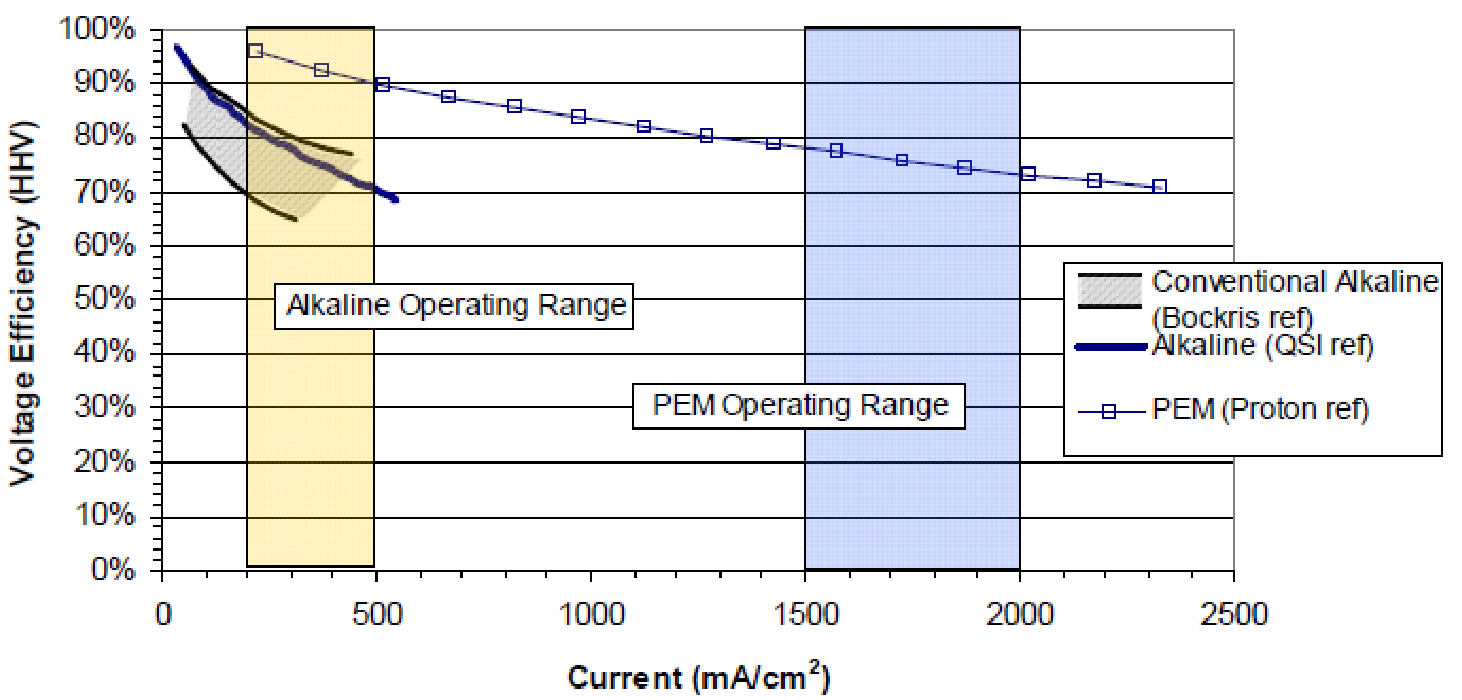
\includegraphics[width=0.7\linewidth]{content/Grafiken/Ely-Efficiency}
	\caption[Elektrolyseur Spannungseffizienz]{Elektrolyseur Spannungseffizienz \cite{NOWH2}}
	\label{fig:ely-efficiency}
\end{figure}


\section{Stromrichter}
\label{sec:Stromrichter}
Allgemein kann man jede Schaltung die zur Strom- und Spannungsversorgung dient als Stromrichter bezeichnen, dabei wird unterschieden zwischen Wechsel- und Gleichspannungsvarianten. Außerdem kann bei Netzanwendungen in gesteuerte, Netz-gesteuerte und ungesteuerte unterschieden werden, sowie die Umsetzung einer \gls{PFC} betrachtet werden. 
		\subsection{Gleichrichter}
		Ein Gleichrichter wird verwendet, um aus einer Wechselspannung eine Gleichspannung zu erzeugen. Die einfachste Form ist der Diodengleichrichter, dieser kann für einphasige Wechselspannung durch eine einzelne Diode realisiert werden. Jedoch würde so nur die halbe Periode des Sinus am Ausgang zur Verfügung stehen, da die Diode nur während der positiven Halbwelle Leitet. Dies lässt sich durch die Ergänzung zum Brückengleichrichter mit vier und für dreiphasige Anwendungen mit sechs Dioden ausgestattet ist.\\
		Anhand des Diodengleichrichters wird schnell klar, dass eine solche Schaltung nur bedingt für einen gewünschten Stromverlauf sorgt. In Abbildung \ref{B6DiodRect} sind Netzspannung und Strom dargestellt, der Stromverlauf zeigt Starke Sprünge und der gewünschte Sinusförmige Verlauf ist nur schwer erkennbar. Außerdem lässt sich mit dieser Schaltung die Ausgangsspannung sowie der Strom nicht variieren.
		\begin{figure}[H]
			\centering
			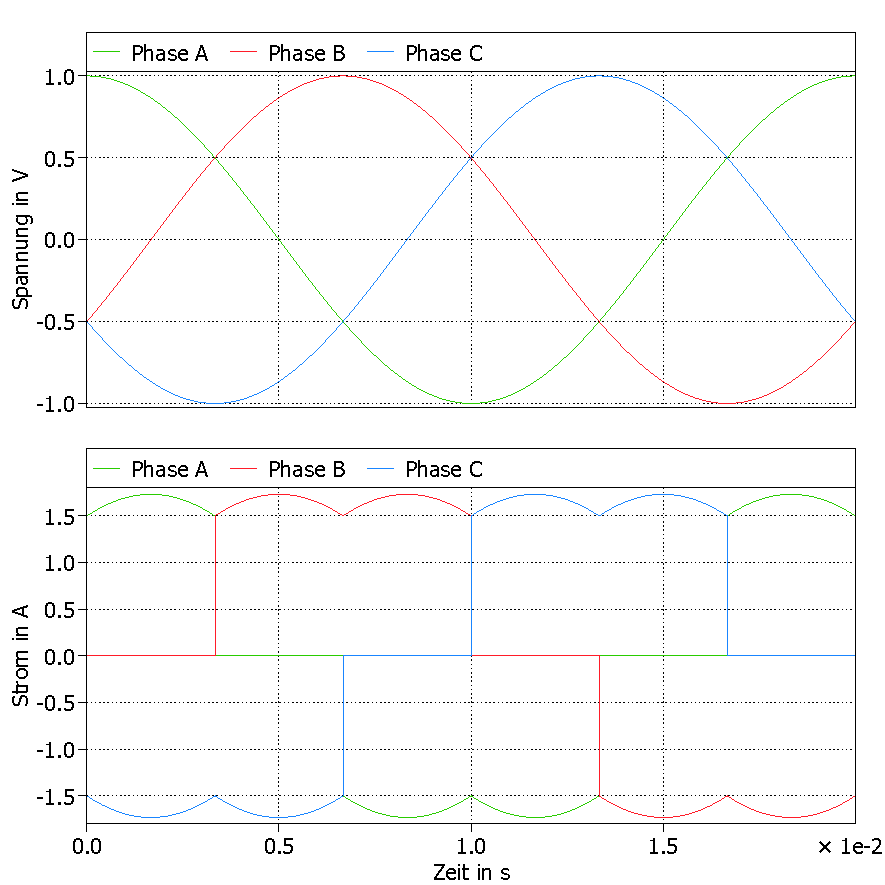
\includegraphics[width=0.7\linewidth]{content/Grafiken/B6-Diodengleichrichter-Eingangsverlauf}
			\caption{Strom und Spannungsverlauf am B6 Diodengleichrichter}
			\label{B6DiodRect}
		\end{figure}
		
		Für Elektrolyseanlagen mit mehreren Megawatt Leistung müssen Zwangsweise Leistungshalbleiter parallelisiert werden, da bei Spannungen bis 1000 V die Ströme für einzelne Halbleiter zu hoch sind. Außerdem bietet die Parallelisierung durch Interleaving und Phasenverschiebung deutliche Vorteile für die Verzerrung und damit Filterung. Durch Thyristor basierte Schaltungen können große Leistungen effizient umgesetzt werden, jedoch führen diese zu deutlichen Verzerrungen des Stromverlaufs und schlechterem Leistungsfaktor. Daher benötigen diese passive oder aktive Filter, welche die Systemkosten erhöhen \cite{HydrogenElectronicTopologies}.
		Als Alternative dazu werden \gls{AFE} Gleichrichter eingesetzt diese bieten deutlich geringere Verzerrungen und völlige Freiheit bei der Regelung des Eingangsstroms. Daher können die Filter und Blindleistungskompensation in diesem Fall eingespart werden \cite{HydrogenElectronicTopologies}.
		
		\subsection{DC-DC Wandler}
		Der Hoch- und Tiefsetzsteller sind essenzielle Topologien und bestehen im wesentlichen aus einer Diode, einem Schalter und einer Induktivität. 
			
		\subsection{Power Factor Correction}
			Die \gls{PFC} ist eine nötige Maßnahme um den Blindleistungsanteil im Netz zu reduzieren 
			The front-end circuit concept of the H3R system was first introduced in late 90s by Jantsch and Verhoeve,

In gängigen Gleichrichtersystemen werden getrennte Einheiten bestehend aus einer dreiphasigen PFC-Gleichrichterschaltung und einem Gleichspannungswandler (DC/DC-Buck-Wandler) eingesetzt, um die Anforderungen zu erfüllen. Die Regelung der beiden Wandlerstufen ist in der Regel entkoppelt, wobei der Gleichrichter sinusförmige Netzströme zieht und der nachfolgende DC/DC-Wandler die Spannung auf den erforderlichen Ausgang anpasst. Auf der Suche nach kompakten und leichten Systemen sind hohe Schaltfrequenzen notwendig, was jedoch zu erhöhten Schaltverlusten und verringerter Wandlereffizienz führen kann. Um dies zu adressieren, werden fortgeschrittene Modulationstechniken wie Einfügen der dritten harmonischen und Raumzeigermodulation möglich. Alternativ kann auch Diskontinuierliche Pulsweitenmodulation (DPWM) als Methode zur Reduzierung der Schaltverluste in dreiphasigen PFC-Gleichrichtern verwendet werden, um sinusförmige Eingangsströme und eine konstante Gleichspannung sicherzustellen. Im Gegensatz dazu müssen Einstufen-Wandlersysteme beide Anforderungen gleichzeitig erfüllen, während Zweistufen-Systeme trotz niederfrequenter Spannungsschwankungen im Zwischengleichspannungsnetz eine konstante Ausgangsspannung sicherstellen können.			
			
\section{IAF Rectifier}
Der \gls{IAF} Gleichrichter wurde erstmals vorgestellt in \cite{IAFfirst} im Jahr 1997 . Dieser besteht für den Hauptleistungspfad aus einem Diodengleichrichter, um sinusförmige Ströme in allen drei Phasen einzuprägen wird dieser durch ein Netzwerk aus bidirektional Sperrenden Leistungshalbleitern ergänzt, welche einen Strom in den Gleichrichter einprägen. Durch die Integration des Filters in den Leistungspfad, kann die Kompensation effizienter funktionieren. Aufgrund des ungesteuerten Diodengleichrichters wird jedoch eine anschließende Spannungsregelung durch einen Tiefsetzsteller benötigt.

\section{1/3 PWM PFC Rectifier}
Bei dieser Topologie handelt es sich um eine gängige Schaltung, welche durch ein neuartiges Modulationsverfahren unter Verwendung von Induktivitäten auf der Netzseite eine Reduzierung der Schaltverluste bewirkt und Blindleistung ermöglicht. Das Verfahren wurde ausführlich von Menzi, Bortis und Kolar beschrieben \cite{13PWMPFC}.

\includesvg{content/Grafiken/B6_Buck}



\section{Leistungshalbleiter}
Halbleiter sind prinzipiell alle Komponenten mit mindestens einem PN-Übergang, wenn diese größere Leistungen Schalten können, werden sie als Leistungshalbleiter bezeichnet. Dazu sind für die verwendete Topologie, neben der klassischen Diode, MOSFET relevant. Diese lösen in der Leistungselektronik aktuell den verbreiteteren IGBT ab aufgrund der günstiger gewordenen Silicium Carbide Variante \cite{SiCTrend}. Die Vorteile dieser neuen Technologie liegen in der Ermöglichung höherer Schaltfrequenzen, dies wiederum ermöglicht die Reduzierung der Energie welche in den Induktiven Komponenten gespeichert werden muss und somit Kostenersparnis. 

\section{Induktivitäten}

\section{Simulationssoftware}
Zur Bewertung und Betrachtung der Umsetzbarkeit, der Topologien ist es nötig diese in einer Umfassenden Simulation zu betrachten. Dies ermöglicht es die Funktionalität und den Einfluss der Parameter im direkten Zusammenspiel zu untersuchen. Insbesondere das Verhalten für Systemdienstleistungen, wie Phasenverschiebung und die dadurch beeinflusste Verteilung der Verlustleistungen sollen als Entscheidungsgrundlage dienen. 

	\subsection{PLECS}
	Die Software \gls{PLECS} aus dem Haus PLEXIM wird als Integration in MATLAB mit Simulink verwendet.  Diese ermöglicht die Modellierung von Schaltungen mit der Betrachtung des Thermischen Verhaltens durch elektrische Modelle der Verlustleistung. Dazu wird die Energie im Schaltvorgang sowie im Durchgeschalteten Zustand in der Schaltung berücksichtigt. Dies ermöglicht es die Verlustleistung innerhalb der Halbleiter zur betrachten und damit den Aufwand für die Kühlung und eine Abschätzung der Schaltungseffizienz. 